\section{The Bayesian Method}
At the second attempt, we use Bayesian probability to determine which semantic model is chosen. This chapter shows the introduction of Bayesian probability, the method of model adaptation. Besides, we investigate the issue of this method.

To avoid wasting lots of resources on unexpressive models, we need a more advanced model adaptation technique. That is to say, the model adaptation should invest the limited computing resources in the promising model more often and explore different models when the most expressive model is uncertain. For this purpose, the probability of choosing the model is measured in terms of the Bayesian posterior probability.

Although this method can work theoretically, it doesn't work as expected in our experiments. We will describe this phenomenon in the follow section.

 
\subsection{The Bayesian Posterior Probability}
In Bayesian inferencing, the posterior probability~\citep{lee2012bayesian} of a random event is the conditional probability that is assigned after the relevant evidence is taken into consideration. Similarly, the posterior probability distribution is the probability distribution of an unknown quantity, treated as a random variable, conditional on the evidence got from an experiment.

%The posterior probability is the probability of the parameter $\theta$ given the evidence $X:P(\theta|x)$. It contrasts with the likelihood function, which is the probability of the evidence given the parameters: $p(x|\theta)$. Let us have a prior belief that the probability distribution function is $p(\theta)$ and observation $x$ with the likelihood $p(x|\theta)$, and then the posterior probability is defined as
%\begin{equation}
%p(\theta|x) = \frac{p(x|\theta)p(\theta)}{p(x)}
%\end{equation}.

In our case, we want to measure the posterior probability of a semantic model given the permutation problem $P$: $Pr(M|P)$. Assuming all semantic models are equally probable, the posterior is proportional to its likelihood $Pr(P | M)$, which can be easily calculated as $ Pr(P | M) =
    \prod_{\forall i \in P}{Pr(i|M)}\text{,}$ 
where $P$ is the population containing individuals and $Pr(i|M)$ is the conditional probability of a specific individual in the population given the semantic model. 



\subsection{Model Adaptation}
{\LinesNumbered
\begin{algorithm}[htbp]
     \KwIn{The initial population $P$,\newline
    The semantic model set $\mathbb{M}$
    }
    \KwOut{The offspring population $O$}


        build each semantic model $m \in \mathbb{M}$ for $P$\;
        measure the posterior of each model $m \in \mathbb{M}$ according to $P$\;
        offspring population $O := \{\}$\;
        \ForEach{$p \in P$}{
            choose a model $m$ according the probability distribution $P(\mathbb{M})$\;
            let $p$ be the template, generate a new individual $c$ by model $m$\;
            \If{$c$ is better than $p$}{ $O$ := $O \cup \{c\}$\; } 
            \Else{$O$ := $O \cup \{p\}$\; }

        }
        return $O$\;
    \caption{The Bayesian Method}
    \label{alg:bayesian_method}
\end{algorithm}}
Since we have the method to measure the posterior of the semantic models, this method can be applied to the model adaptation. For the preliminary study, the posterior of the semantic model is directly used as the probability of choosing the model to generate new individuals.

Formally, for each model $m \in M$, where $M$ is the set of the models the system has, $Pr(m)$ is the probability that the model $m$ is chosen as the most expressive model to generate new individuals among the model set $M$. The probability is defined as
\begin{equation*}
    Pr(m) = \frac{q_m}{\Sigma_{j \in M} {q_j} }\text{,}
\end{equation*}
where $q_j$ is the posterior of the semantic model $j$. 

For model adaptation, the Bayesian method chooses a model before the sampling phase. Because the population reflect the semantics of the permutations as the population evolves, the posterior of the expressive models for the specific permutation problem increases. Hence, these models for the specific permutation problem have more chance to generate new individuals, while the other candidate models still have little chance.

The pseudo code is in Algorithm \ref{alg:bayesian_method}. The model adaptation stage between model building and sampling. Let the population size be $N$. In every generation, the Bayesian method  iterates the whole population to make each individual template for generating new individual, and then keeps the better one between new generated offspring and the template. This difference accelerates the population reflecting the problem semantics, due to the population moves toward the high fitness solutions.  


\subsection{Empirical Study}
In this subsection, the performance of the Bayesian method is investigated. In practice, the conditional probability of the population given the model will be expressed in logarithm for computation convenience, since the value is too small for the float-point number in computer. 

For the experiment purpose,  TSP and the flat problem are tested. The objective value of the flat problem is a constant, no matter the permutation is. Hence, the posterior of the solution on the flat problem is independent from the semantic models. 

\begin{figure}[t]     
    \begin{subfigure}{1.0\textwidth}
        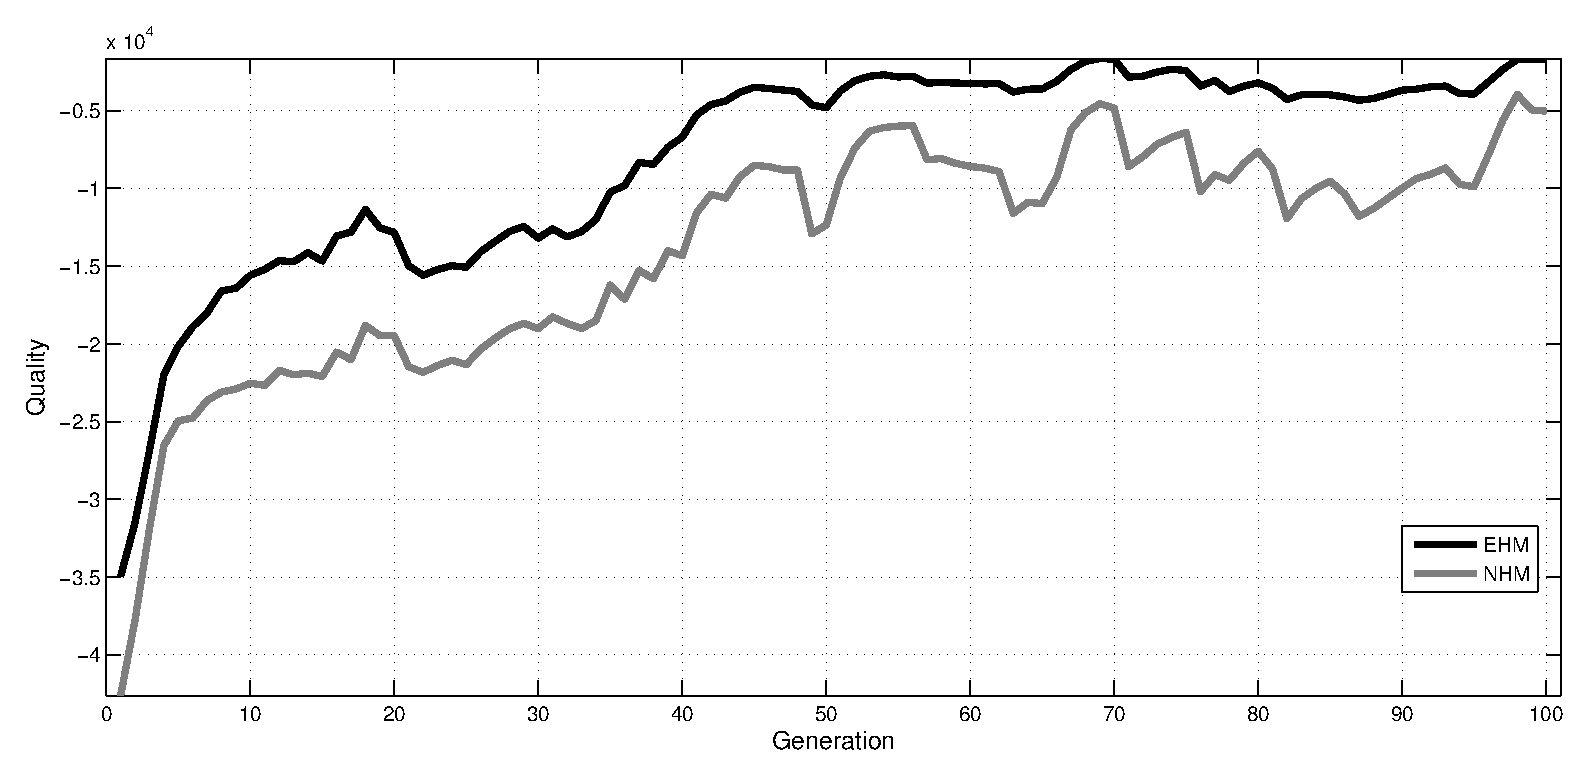
\includegraphics[width=1.0\textwidth]{bayesian_tsp.eps}
        \caption{TSP, eil51, $L=51$, $N=1000$}
    \end{subfigure}\\

    \begin{subfigure}{1.0\textwidth}
        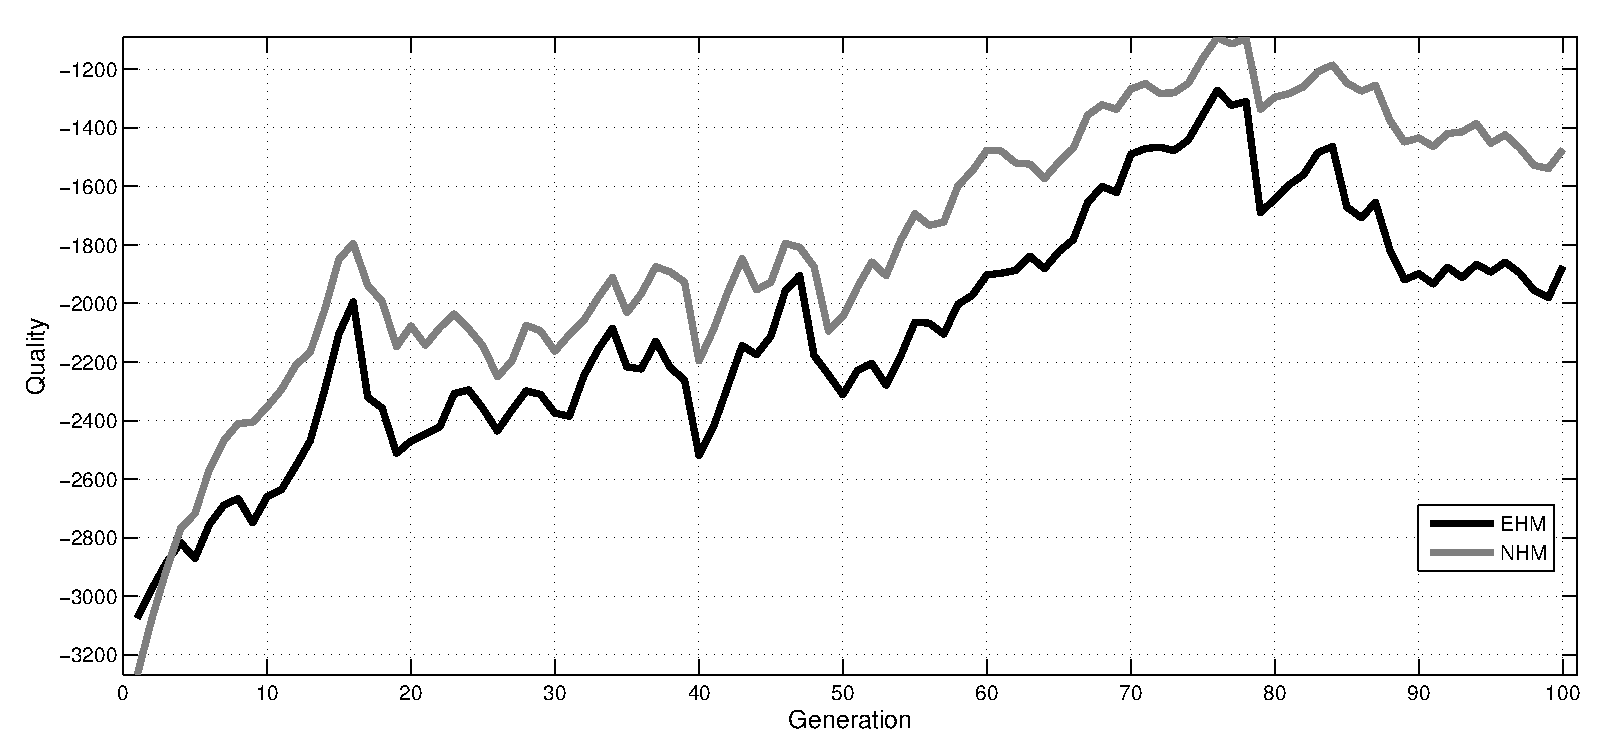
\includegraphics[width=1.0\textwidth]{bayesian_flat.eps}
        \caption{Flat, $L=50$, $N=100$}
    \end{subfigure}
    \caption{(Temp)The posterior of the semantic model, tournament selection $S=2$ }
    \label{fig:bayesian_quality}
\end{figure}

In the experiment of the Bayesian method, EHM and NHM are used. The population size $N$ is $1000$ for TSP and $N$ is 100 for the flat problem. We perform independent 10 runs on each instance. The problem size of the flat problem is $50$. The instance eil51 of TSP has been used in this empirical study \footnote{\textbf{TSPLIB} http://www.iwr.uni-heidelberg.de/groups/comopt/software/TSPLIB95/}.%The experiment settings are as the follows:
%\begin{itemize}
    %\item repeat 10 times,
   % \item the NHM and the EHM are used,
   % \item population size $N=1000$ for TSP and $N=100$ for the flat problem,
   % \item the bias ratio $B_{ratio} = 0.0000$,
   % \item template technique is used,
   % \item the cut-point number is 3 for template.
%\end{itemize}
 

Figure \ref{fig:bayesian_quality} shows the posterior of the semantic models in term of the logarithm the conditional probability of the population given the semantic model. The higher the posterior, the better the model describes the problem. As can be seen, at the beginning of the trials on the flat problem and TSP, the posterior of NHM is lower than that of EHM. After 5 generations, the posterior of NHM becomes higher than that of EHM on the flat problem and remains higher until the trial ends. 

Although the posterior of EHM in TSP is higher than that of NHM as we expected, the posterior of NHM on TSP grows faster than EHM as the population evolves. To demonstrate the phenomenon, we test the flat problem in our experiments. The posterior of the both models on the flat problem is not identical as we expected. This result shows that NHM is more sensitive than EHM to population changes.

Of course, these effects of the phenomenon can be eliminated by preproduce. However, introducing new techniques to the Bayesian method for balancing different models also increase the cost of adding new models into this system, so we attempt to develop another method in the follow chapter.